% !TEX root = ../presentation.tex


\subsection[Constrained Attitude Control]{Constrained Attitude Control}

\subsubsection[Attitude Background]{Attitude Background}
% Results from 2016 ACC

\begin{frame}{Spacecraft Orientation}\label{slide:attitude_control} %-----------------------------%

\begin{itemize}

    \item \Emph{Attitude Representation}: rotation matrix from body to inertial frame \hyperlink{slide:attitude_kinematics}{\beamergotobutton{Attitude Kinematics}}
     \[\SO =  \{R\in\R^{3\times 3}\,|\, R^TR=I,\;\mathrm{det}[R]=1\} . \]
    \item Rigid body attitude dynamics:
    \begin{gather*}
        J\dot\Omega + \Omega\times J\Omega = u+W(R,\Omega)\Delta , \quad \dot R = R\hat\Omega .
    \end{gather*}

    \item Sensor and obstacles defined by unit vectors in \( \R^3 \) 
        \begin{itemize}
            \item Body fixed sensor: \( r \in \S^2\)
            \item Inertially fixed hazard: \( v \in \S^2 \)
        \end{itemize} 
    \item Hard cone constraint: \( r^T R^T v \leq \cos \theta \)
    
\end{itemize}

\note[itemize]{
    \item Obstacle described as a cone around the direction of avoidance
}
\end{frame}   %-----------------------------%

\subsubsection[Attitude Control]{Attitude Control}

\begin{frame}{Control Objective} %---------------------------------------%

    \begin{block}{Nonlinear Control Design}
        Design control input \( u \) that stabilizes system from initial attitude \( R_0 \) to desired attitude \( R_d \) while avoiding obstacles
    \end{block}
    \pause
    \begin{itemize}
        \item Avoid drawbacks of other approaches 
        \begin{itemize}
            \item \Emph{Geometric control} - analysis is conducted directly on \( \SO \) 
            \item \Emph{Barrier function} - allows for arbitrary amount of constraints
            \item \Emph{Efficient } - real time feedback control
            \item \Emph{Stability} - Lyapunov analysis gives rigourous stability proof
            \item \Emph{Adaptive} - handles system uncertainties
        \end{itemize}
    \end{itemize}
\end{frame}

\begin{frame}{Configuration Error Function} %-----------------------------%
\only<1>{
\begin{itemize}
    \item Error function quantifies ``distance'' to desired attitude
    \begin{align*}
            \Psi(R, R_d) = A(R, R_d) B(R) .
    \end{align*}
    \item Combination of attractive and repulsive terms   
\end{itemize}
\begin{gather*}
    A(R, R_d) = \frac{1}{2} \tr{G \left( I - R_d^T R\right)} . \\ \\
    B_i(R) = 1 - \frac{1}{\alpha_i} \ln \left( - \frac{ r^T R^T v_i - \cos \theta_i}{1 + \cos \theta_i}\right) .
\end{gather*}     
}

\only<2>{
    \begin{itemize}
        \item Attractive well at the desired attitude
    \end{itemize}
    \begin{align*}
        A(R,R_d) = \frac{1}{2} \tr{G \left( I - R_d^T R\right)} .
    \end{align*}
    \begin{center} 
        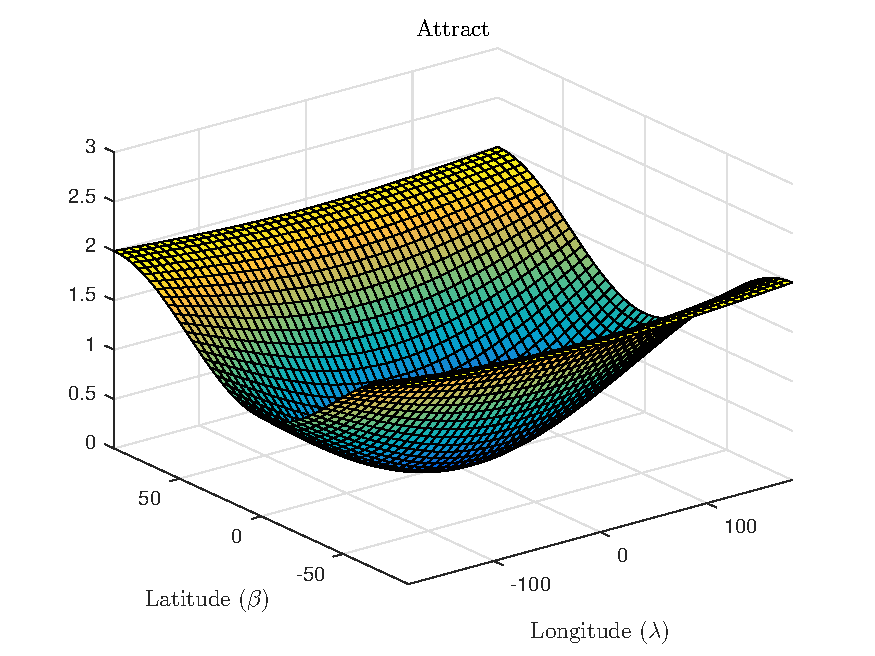
\includegraphics[height=0.6\textheight]{figures/2016ACC/attract_error.pdf}
    \end{center}
}

\only<3>{
    \begin{itemize}
        \item Define a barrier around obstacles
    \end{itemize}
    \begin{align*}
        B_i(R) = 1 - \frac{1}{\alpha_i} \ln \left( - \frac{ r^T R^T v_i - \cos \theta_i}{1 + \cos \theta_i}\right).
    \end{align*}
    \begin{center}
        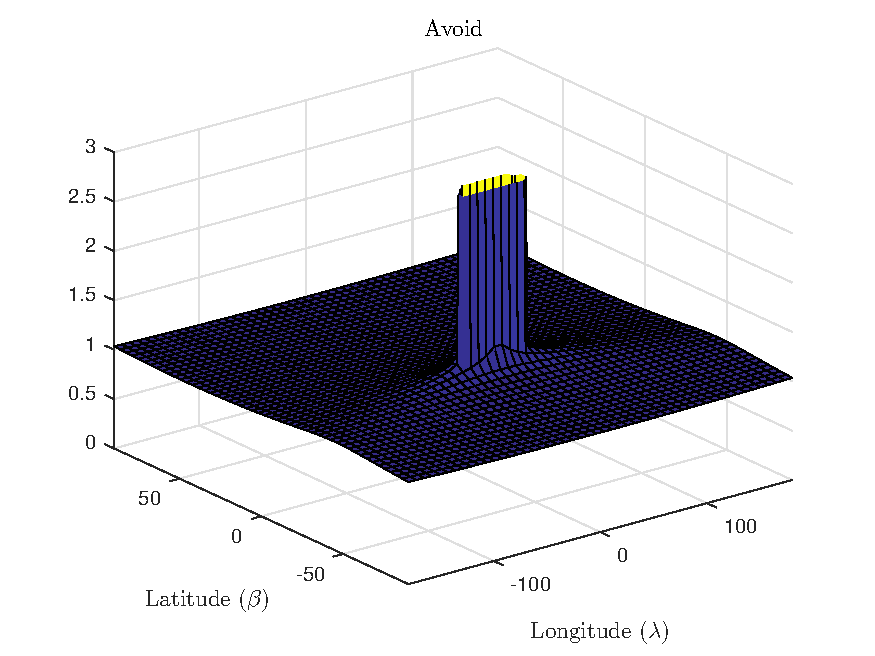
\includegraphics[height=0.6\textheight]{figures/2016ACC/avoid_error.pdf}
    \end{center}

}

\only<4>{
    \begin{itemize}
        \item Configuration error: \( \Psi : \Q \times \Q \to \R \) with control chosen to follow slope of \( \Psi \) to minimum at \( R_d\)
    \end{itemize}
    \begin{align*}
        \Psi(R, R_d) = A(R,R_d) B(R) .
    \end{align*}
    \begin{center}
        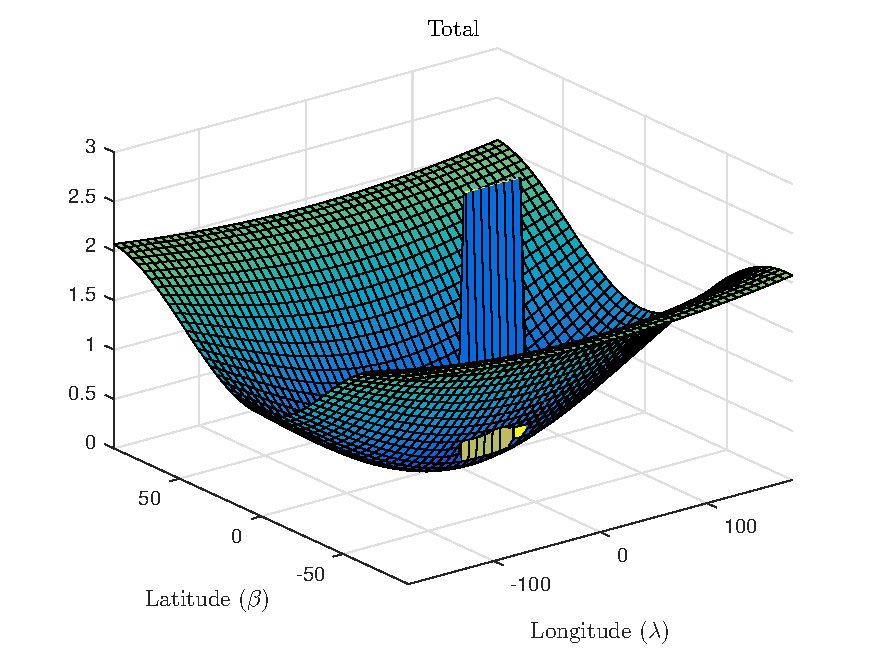
\includegraphics[height=0.6\textheight]{figures/2016ACC/combined_error.pdf}
    \end{center}
}

\note[itemize]{
    \item First step in control design is the selection of an error function
}
\end{frame}   %-----------------------------%

\subsubsection[Simulation]{Numerical Simulation}
\begin{frame}{Numerical Simulation} %-----------------------------%

\begin{itemize}
    \item Simulate a S/C completing a yaw rotation
    \item Single obstacle in the path of sensor
\end{itemize}

\begin{center}
    \animategraphics[controls,autoplay,loop,width=0.5\textwidth]{8}{animation/2016ACC/single_noavoid/single_noavoid-}{0}{99}~
    \animategraphics[controls,autoplay,loop,width=0.5\textwidth]{8}{animation/2016ACC/single_avoid/single_avoid-}{0}{99}
\end{center}

\end{frame}%-----------------------------%

\begin{frame}{Multiple obstacles}%-------------------------------------%

\begin{itemize}
    \item Easily handle multiple arbitrary constraints 
    \begin{align*}
        \Psi = A(R) \bracket{1 + \sum_i C_i(R)} \quad C_i = B(R) - 1
    \end{align*}
\end{itemize}

\begin{center}
    \animategraphics[controls,autoplay,loop,width=0.5\textwidth,height=0.5\textheight,keepaspectratio]{8}{animation/2016ACC/multiple_avoid/multiple_avoid-}{0}{99}
\end{center}

\end{frame}%---------------------------------------%

\subsubsection[Experiment]{Hardware Implementation}

\begin{frame}{Hexrotor Experiment} %-----------------------------%
\begin{itemize}
    \item Attached to spherical joint to allow only attitude dynamics
\end{itemize}
\begin{center}
    \href{https://youtu.be/dsmAbwQram4?t=20s}{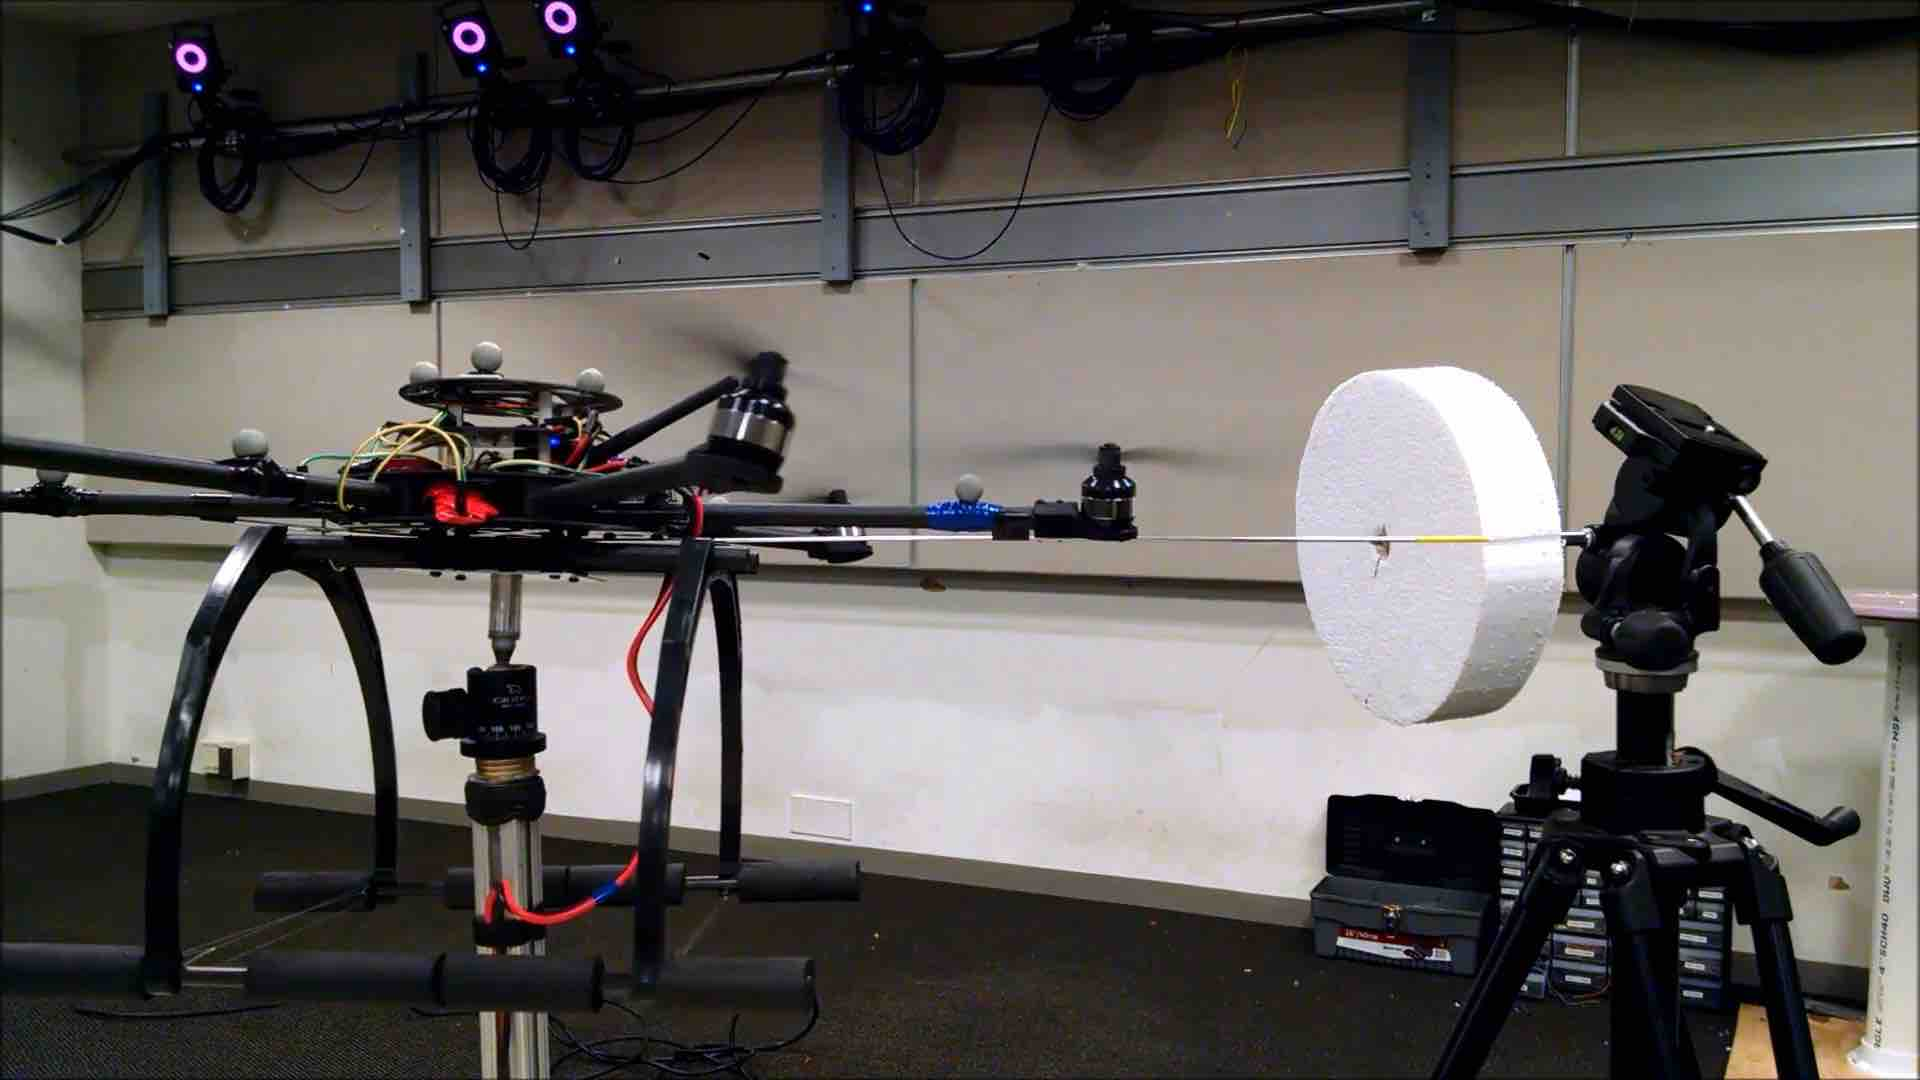
\includegraphics[height=0.7\textheight]{figures/2016ACC/hexrotor}}
\end{center}
\end{frame}   %-----------------------------%
